% Considera��es finais
\chapter{Considerações finais}

\section{Principais dificuldades}

A maior dificuldade encontrada durante todo o desenvolvimento do sistema foi a implantação, ou seja, fazer com que a plataforma fosse disponível na web. Como foi deixado claro durante todo o decorrer do trabalho, foi optado por utilizar os serviços em nuvem da Amazon para realizar o deploy. Inicialmente, foi estudado o EC2, mas logo se percebeu que o trabalho era totalmente manual, com a criação de VPCs, máquinas virtuais, banco de dados (RDS), domínios (Route53) e etc, o que fez com que outras alternativas fossem buscadas. 

Outras duas opções viáveis, também da Amazon, foram estudadas. A primeira foi o ElasticBeanstalk, que na sua essência tem a função de abstrair esse processo manual citado, apenas realizando pequenas especificações, como o banco de dados, qual linguagem de programação foi utilizada, dentre outras. A segunda foi o CodeStar que abstrai ainda mais o processo, adicionando a opção de criação de templates prontos, isso quer dizer, é possível escolher uma aplicação pronta para uso com Rails, com um domínio, com integração ao GitHub e utilizando DevOps.

Nesses dois cenários foram realizados diversas tentativas (utilizando Docker inclusive), mas sem sucesso. Com isso, foi concluído que essas abstrações proporcionadas, apesar de serem úteis e eficazes para pequenas aplicações, quando utilizadas em sistemas um pouco mais complexos e com dependências maiores, acabam por atrapalhar, pois as falhas que surgem não se tornam explícitas, mesmo havendo alguns logs. Com esse empecilho, outras práticas programadas, como a utilização do docker em produção e o integra contínua não pode ser feita.

Visto isso, foram buscadas novas alternativas fora do ambiente Amazon. Foi tentando com o Heroku\footnote{https://www.heroku.com/} e DigitalOcean\textit{https://www.digitalocean.com/}, sem sucesso também. O erro encontrado em todas as tentativas era referente ao \textit{asset pipeline}, que segundo a documentação do Ruby on Rails “é o responsável por fornecer uma estrutura para concatenar, minificar ou compactar ativos JavaScript e CSS. Ele também adiciona a capacidade de gravar esses recursos em outros idiomas e pré-processadores, como CoffeeScript, Sass e ERB”. O erro é que esses assets não estavam sendo processados em produção automaticamente.

Divulgar o trabalho para estrangeiros foi outro problema encontrado, pois não houve um grande engajamento em relação à ideia. Mas esse fato tem um peso negativo menor, pois o BNativus foi desenvolvido essencialmente para ajudar os brasileiros, mas precisamente os estudantes dos institutos federais. Posteriormente, se houver uma boa aceitação.


\section{Trabalhos futuros}

A essência da ideia já foi desenvolvida, todavia ainda há algumas ideias a serem implantadas. Algumas delas podem ser vistas na figura 6, na coluna de \textit{ideias} e \textit{todo}. Acrescentá-las a aplicação agregaria novas funcionalidades e melhorias, aumentando as chances de atrair novos usuários ao sistema. Mas o que foi feito foi apenas um MVP, com o mínimo de funcionalidades, pois não iria adiantar desenvolver todas as funcionalidades, se não houvesse pessoas para utilizar. Portanto, essas ideias ficaram como um trabalho futuro, para que no momento em que começar a ser usado de fato, as modificações pudessem ser acrescentadas aos poucos. Por isso foi deixado claro que essa é uma versão beta, com o básico de funcionalidades.

Receber feedback dos usuários sobre o sistema é uma forma dessas novas ideias surgirem, afinal, o software foi desenvolvido para eles. Além disso, é possível perceber também se o rumo que o software está seguindo é aprovado pelos usuários. Caso eles não se sentirem confortáveis usando, irá resultar em uma diminuição de acessos ou até mesmo o abandono. Visando essa comunicação foi adicionado ao site um botão de sugestões, no lado direito do cabeçalho. Ele direciona para um formulário que contém algumas informações perguntas e um espaço de sugestão, onde o usuário pode deixar a sua opinião, positiva ou negativa, sobre o sistema. Tudo será coletado e irá ser analisado, a fim de adquirir novas ideias a serem adicionadas no futuro.

\begin{figure}[!htb]
	\centering
  	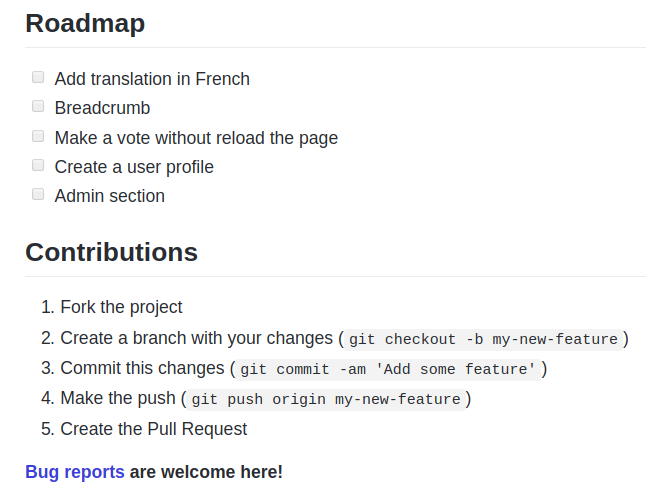
\includegraphics[scale=0.5]{src/imagens/readme.png}
  	\textsf{\caption{Comentário dentro da plataforma BNativus}}
  	\label{fig:FiguraTeste}
\end{figure}

Parte dessas ideias estão listadas no repositório do GitHub, como é demonstrado na imagem acima, dessa forma alguém que se interessar pelo projeto pode seguir o guia de contribuição, e adicionar novas funcionalidades. Isso é possível pois o BNativus possui seu código aberto, o que quer dizer que qualquer pessoa, com uma conta no GitHub, pode realizar modificações no projeto. A ideia é que o sistema seja voltado para a comunidade, e que ela possa o manter também.

Apesar dessa ideia colaborativa, é importante ter alguma espécie de renda, uma vez que para manter um sistema web no ar, algumas taxas são cobradas, como servidor e domínio. É previsto que essa seja uma preocupação, apesar de até o momento não ser, pelos custos serem baixos. A melhor forma encontrada para ganhar dinheiro a partir do sistema no futuro foi criar um tipo de moeda de troca. Ela funcionaria da seguinte forma: se um canadense deseja praticar o português, ele poderia ir até a plataforma e se comunicar por um tempo X com um brasileiro, este último, por sua vez, ganharia um tempo equivalente para conversar com outras pessoas no idioma que deseja praticar.

\section{Conclusão}

    Quando o sistema aqui apresentado foi idealizado, houve uma preocupação de colocar em prática tudo o que foi aprendido durante o curso e nas experiências extra curriculares, como o estágio. O máximo dessas tecnologias e práticas foram utilizadas, havendo uma boa integração, de modo geral, entre elas sendo possível, no fim, construir todo o escopo planejado no período estabelecido, e ter o MVP.
	
	Apesar desta organização, foi concluído que é necessário ter um cuidado ainda maior nas escolhas das tecnologias, sempre almejando o final, quando for feita a implantação e os usuários irão usar de fato o sistema. Essa falta de preocupação ocasionou problemas em colocar o sistema em produção, o que impossibilitou que o sistema fosse testado com usuários reais prejudicando, assim, a validação da ideia. Como foi explicado, houve a busca  por alternativas para ser realizado a implantação, mas sem sucesso. Isso não implica que a AWS, serviço escolhido para realizar o deploy, não funciona. Isso quer dizer que provavelmente houvesse formas mais simples de realizar a implantação de aplicações Rails ou que exista uma abordagem que funcionaria para o caso do BNativus, mas que não foi encontrada nas pesquisas feitas.

	Contudo, foi provado que há um público que utilizaria o sistema, o que trouxe a motivação de continuar o trabalho. Posteriormente, irão ser feitas novas tentativas, com base em novas pesquisas e novas abordagens de implantação, havendo um maior cuidado.
